\section{Rank Sort algorithm}
\subsection*{a) Propose an algorithm with a running time of $O(log N)!$}
Consider $n-1$ processors for each element dedicated to the computation of its rank as follows (comparison need not be done with the element it self hence why only $n-1$ processors are needed rather than $n$):

\[
\begin{array}{cccc}
a[0]< a[i] & \dots  & a[n-1]< a[i] & \# P = n-1  \\ 
a[0]< a[i+1] & \dots  & a[n-1]< a[i+1] & \#P = n-1 \\ 
\vdots  & \vdots  & \vdots  & \vdots 
\end{array}
\]

After which every processor holds either a 0 or a 1. Summation of all $n-1$ columns for each row (i.e. for each i) yields the rank of element $i$. Rank of element i = $\sum_{k=1}^{n-1} P_{ik}$. Using recursive doubling this is done in $\log(n)$ time.

\subsection*{b) How many processors are needed? What is the processor efficiency?}
$n(n-1) \approx n^2$ processors are needed. We suppose that time requiered for comparison of two numbers is roughly equal to that of summation of two numbers = $t_{comp}$.  On one processor the time would be $t_1 = t_{comp}\cdot n^2$. On $n^2$ processor the required time is $t_P = n\cdot t_{comp} + t_{recursive\ doubling} =  n\cdot t_{comp} +\log_2(n)(2(t_{startup}+t_{data})+t_{comp}) $ The efficiency is:

\begin{gather*}
E = \frac{t_1}{t_P\cdot P} = \frac{n^2t_{comp}}{ n^2(nt_{comp}+ \log_2(n)(2(t_{startup}+t_{data})+t_{comp}))} =\\ \frac{t_{comp}}{nt_{comp}+ \log_2(n)(2(t_{startup}+t_{data})+t_{comp})}
\end{gather*}

Which tends rather quickly towards 0 as $n$ increases. This algorithm is really unefficient.

\subsection*{c) Would you use this algorithm in practice? Why or why not?}

Given that $n$ will usually be very large and since we want to use parallel computing, the computation would require far too many processors. Since we are very likely not to have that many processors available, it would be impossible to actually use it.


\section{Odd-Even Transposition Sort as one SPMD program}

The code is not correct, but almost. In order to prevent deadlocks, half of the processes must first receive a message before sending it.

Furthermore, process $0$ cannot receive from $-1$, nor can $n-1$ send to $n$.

Here is a corrected version of the algorithm:

\begin{lstlisting}
evenprocess = (rem(i,2) == 0);
evenphase = 1;
for step = 0:N-1
    if (evenphase & evenprocess) | (~evenphase & ~evenprocess)
        if(p < n-1)
            send(a, i+1);
            receive(x, i+1);
            if x < a
                a = x;
            end
        end
    else
        if(p > 0)
            receive(x, i-1);
            send(a, i-1);
            if x > a
                a = x;
            end
        end
    end
    evenphase = ~evenphase;
end
\end{lstlisting}


\section{Odd-Even Transposition Sort}
\subsection*{a) Implementation and correctness for a small $N$ and a small number of processors}
Below is the result of our algorithm for $P = 7$ and $N = 32$. 4 processes have $I = 5$ whereas the 3 last processes have $I = 4$.

\begin{verbatim}
mpicc oddevensort.c -o oddevensort && mpirun -np 7 ./oddevensort 32

3 > Local data at step 0 is: 0.92 0.13 0.19 0.26 0.21 
5 > Local data at step 0 is: 0.14 0.96 0.80 0.40 
0 > Local data at step 0 is: 0.84 0.39 0.78 0.80 0.91 
1 > Local data at step 0 is: 0.70 0.81 0.09 0.12 0.35 
2 > Local data at step 0 is: 0.56 0.22 0.39 0.44 0.29 
4 > Local data at step 0 is: 0.27 0.05 0.99 0.08 
6 > Local data at step 0 is: 0.49 0.87 0.59 0.21 
0 > Data received from to 1: 0.13 0.14 0.19 0.21 0.21 
0 > Data received from to 2: 0.22 0.26 0.27 0.27 0.35 
0 > Data received from to 3: 0.39 0.39 0.40 0.44 0.49 
0 > Data received from to 4: 0.56 0.59 0.70 0.80 
0 > Data received from to 5: 0.80 0.81 0.84 0.87 
0 > Data received from to 6: 0.91 0.92 0.96 0.99 
0 > Final result: 0.000 0.046 0.080 0.089 0.121 0.134 0.135 0.191 0.214
0.215 0.225 0.260 0.275 0.275 0.348 0.393 0.394 0.403 0.444 0.487 0.561
0.593 0.701 0.798 0.800 0.810 0.840 0.868 0.912 0.916 0.963 0.993
\end{verbatim}

\subsection*{b) Measure the efficiency of your program by using a large number N (say, N = 107) on P = 1, 2, 3, 4, 8 processors. Provide a plot of the Speedup. Draw conclusions. Do not forget to use optimization switches when compiling and linking.}

Unfortunately, we were unable to use the esubmit command. Therefore we had to resort to the use of 1 virtual node. Thus our data might not be optimal, but the speedup factor should non the less be accurate. Results are presented in graphs below. Judging from the the adapted function, it is reasonable to say that performance is of the form $t = c_1/p+c_2 $.

\begin{figure}[H]
\centering
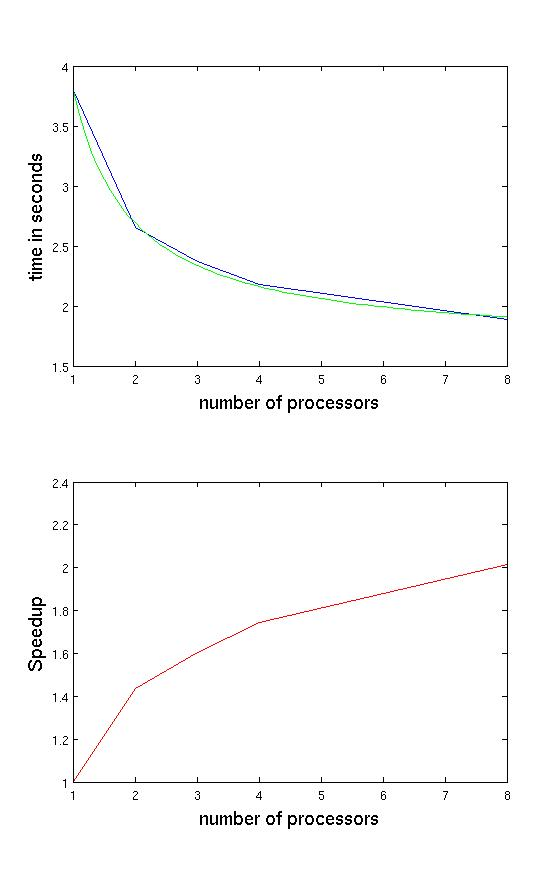
\includegraphics[width=0.9\textwidth ]{img/Data.jpg}
\caption{In blue: mean of 4 measurments for $p = 1,2,3,4,8$ . In green: adapted function $t(p)=2.123t^{-1.066}+1.678$. In red speedup $S_P  \approx T_1/T_P$}
\end{figure}